R-FCN, \cite{DBLP:journals/corr/DaiLHS16}, je potpuno konvolucijski model za detekciju objekata. Budući da modeli s predlaganjem regija postižu bolje rezultate u detekciji od modela bez predlaganja regija, R-FCN, inspiriran arhitekturom R-CNN-a, detekciju radi u dvije faze: 1. predlaganje regija i 2. klasifikacija regija. Međutim, za razliku od Fast R-CNN-a i Faster R-CNN-a koji prilikom detekcije, obavljaju računski skupe operacije za svaku predloženu regiju, R-FCN većinu računskih operacija obavlja samo jednom.
Osnova modela je konvolucijska mreža. Originalno se koristi ResNet-101 (\cite{DBLP:journals/corr/HeZRS15}), ali mogu se koristiti i druge mreže. ResNet se sastoji od 100 konvolucijskih slojeva nakon kojih se nalazi sloj sažimanja srednjom vrijednosti i potpuno povezani sloj. Za potrebe detekcije objekata, odbacuju se sloj sažimanja i potpuno povezani sloj. Konvolucijski slojevi se koriste za izlučivanje značajki koje se dijele između mreže za predlaganje regija i R-FCN mreže. Predložene regije se svrstavaju u jedan od razreda ili se označavaju kao pozadina. U R-FCN mreži,  sve težine koje se optimiziraju su dio konvolucijske jezgre. Izlaz zadnjeg konvolucijskog sloja je $k^2$ mapa rezultata za svaku kategoriju, što je ukupno $k^2(C + 1)$. $k^2$ odgovara mreži dimenzija $k \times k$ na koju se dijeli svaka regija i koja opisuje relativne pozicije. Na primjer, za $k=3$, 9 ćelija ($3 \times 3$) mreže označava relativne pozicije za svaku kategoriju: gore-lijevo, gore-sredina, gore-desno, ... , dolje-desno. R-FCN kao zadnji sloj ima RoI sloj sažimanja osjetljiv na poziciju. Kako bi se informacija o poziciji eksplicitno ugradila u sloj sažimanja, svaka regija se dijeli na $k \times k$ pravokutnika. Za regiju dimenzija $w \times h$, pravokutnici su približno dimenzija $\frac{w}{k} \times \frac{h}{k}$. Unutar $(i, j)$-tog pravokutnika, ($0 \leq i, j \leq k - 1$) definiran je RoI sloj sažimanja ovisan o poziciji koji se primjenjuje samo unutar $(i, j)$-te mape rezultata:
\[
	r_c(i, j | \Theta) = \frac{\sum\limits_{(x,y) \ \epsilon \ bin(i, j)} z_{i, j, c}(x + x_0, y+ y_0 | \Theta)}{n}
\]
U formuli $z_{i,j,c}$ označava mapu rezultata na poziciji $(i, j)$ za razred $c$. Izlaz sloja sažimanja je $k^2$ rezultata za svaki razred koji glasaju nalazi li se objekt tog razreda u predloženoj regiji. Glasanje se radi tako da se izračuna srednja vrijednost $k^2$ rezultata te se na izlazu dobiva vektor dimenzije $(C + 1)$. Za dobiveni vektor se na kraju računa softmax kako bi se dobile vjerojatnosti pripadnosti regije pojedinom razredu tj. pozadini. Arhitektura modela prikazana je na slici \ref{rfcn_arhitektura}, a na slici \ref{rfcn_vizualizacija} je vizualiziran rad modela.
Za trening modela koristi se funkcija pogreške koja se sastoji od pogreške klasifikacije i pogreške regresije
\[
	L(s, t_{x, y, w, h}) = L_{cls}(s_{c^*}) + \lambda [c^* > 0]L_{reg}(t, t^*)
\]
Za pogrešku klasifikacije se koristi unakrsna entropija ($L_{cls} = - \log(s_{c^*})$), a pogreška regresije je ista kao i kod Fast R-CNN-a. $c^*$ je oznaka stvarnog razreda gdje $c^* = 0$ označava pozadinu. Izraz $[c^* > 0]$ poprima vrijednost 1 ako je zadovoljen uvjet $c^* > 0$, tj. pogreška regresije se ne računa ako predviđena regija predstavlja pozadinu. Parametrom $\lambda$ se regulira ravnoteža između pogreške klasifikacije i pogreške regresije, a autori ga postavljaju na $1$.
Budući da je broj računskih operacije koje su specifične za pojedinu predviđenu regiju mali, broj predviđenih regija $N$ ne pogoršava performanse prolaska unaprijed u velikoj mjeri. Stoga se uzima veći broj ($N$) predviđenih regija i za svaku se računa funkcija pogreške. Zatim se uzima $B$ regija s najvećom pogreškom i prolazak unazad se radi samo za te odabrane regije.

 \begin{figure}
	\centering
	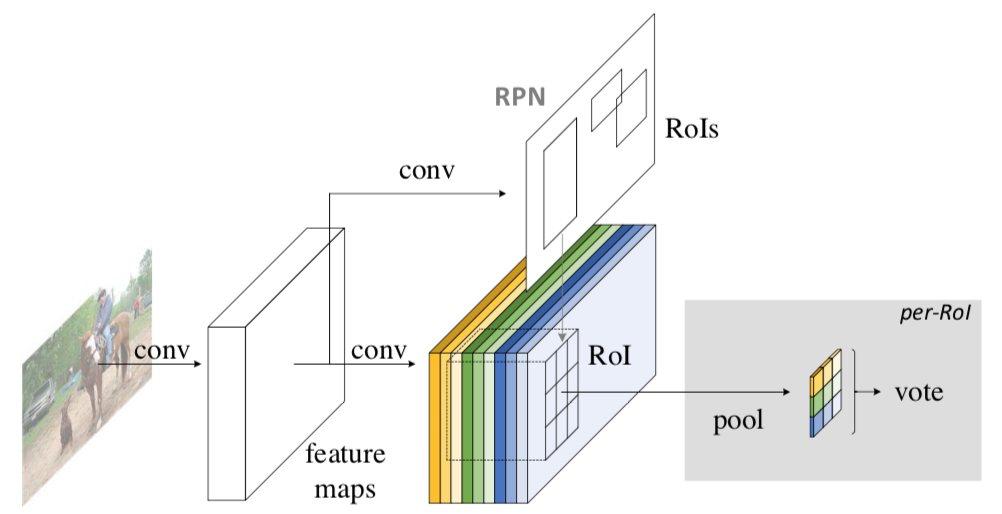
\includegraphics[scale=0.9]{img/rfcn_arhitektura.png}
	\caption{Arhitektura modela R-FCN.}
	\label{rfcn_arhitektura}
\end{figure}

 \begin{figure}
	\centering
	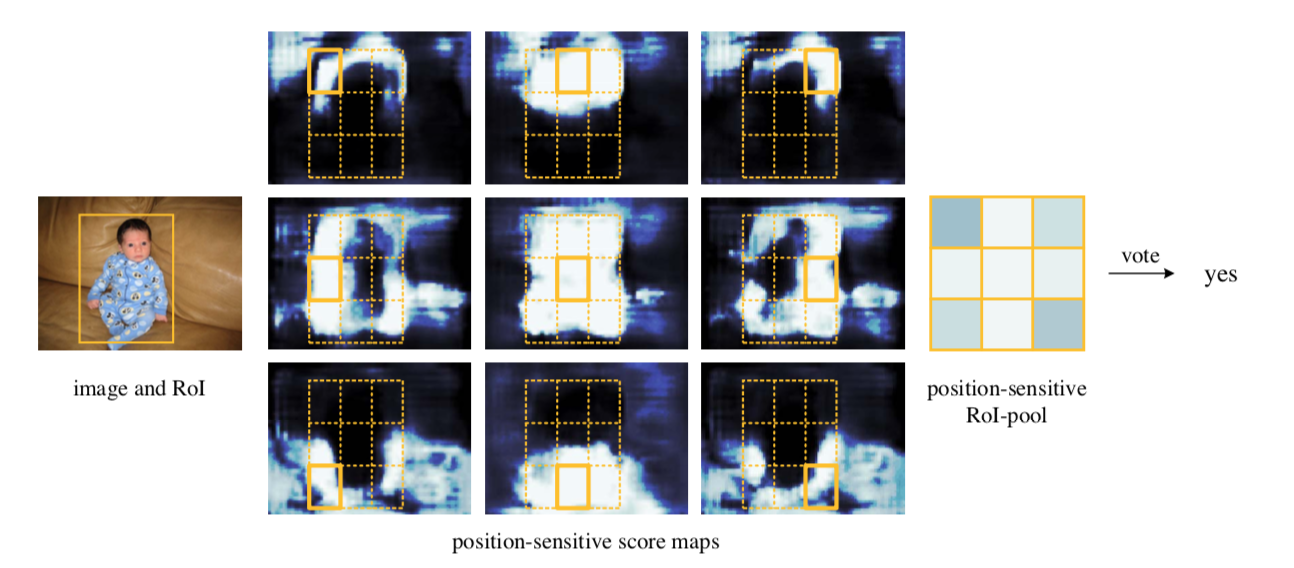
\includegraphics[scale=0.7]{img/rfcn_vizualizacija.png}
	\caption{Vizualizacija detekcije modelom R-FCN. Za predviđenu regiju uzima se dio izlaza zadnjeg konvolucijskog sloja koji odgovara dijelu slike koji pokriva predviđena regija te se dijeli na mrežu $3 \times 3$ i tvori mapu rezultata. Za svaku ćeliju mreže slojem sažimanja ovisnim o poziciji se predviđa nalazi li se odgovarajući dio objekta u toj ćeliji. Na primjer, nalazi li se gornji lijevi dio čovjeka u gornjoj lijevoj ćeliji. Na kraju se glasanje vrši računanjem srednje vrijednosti izlaza sloja sažimanja i donosi se zaključak da se na slici stvarno nalazi čovjek.}
	\label{rfcn_vizualizacija}
\end{figure}